%%%%%%%%%%%%%%%%%%%%%%%%%%%%%%%%%%%%%%%%%
% Beamer Presentation
% LaTeX Template
% Version 1.0 (10/11/12)
%
% This template has been downloaded from:
% http://www.LaTeXTemplates.com
%
% License:
% CC BY-NC-SA 3.0 (http://creativecommons.org/licenses/by-nc-sa/3.0/)
%
%%%%%%%%%%%%%%%%%%%%%%%%%%%%%%%%%%%%%%%%%

%----------------------------------------------------------------------------------------
%	PACKAGES AND THEMES
%----------------------------------------------------------------------------------------

\documentclass{beamer}

\mode<presentation> {

% The Beamer class comes with a number of default slide themes
% which change the colors and layouts of slides. Below this is a list
% of all the themes, uncomment each in turn to see what they look like.

%\usetheme{default}
%\usetheme{AnnArbor}
%\usetheme{Antibes}
%\usetheme{Bergen}
%\usetheme{Berkeley}
%\usetheme{Berlin}
%\usetheme{Boadilla}
%\usetheme{CambridgeUS}
%\usetheme{Copenhagen}
%\usetheme{Darmstadt}
%\usetheme{Dresden}
%\usetheme{Frankfurt}
%\usetheme{Goettingen}
%\usetheme{Hannover}
%\usetheme{Ilmenau}
%\usetheme{JuanLesPins}
%\usetheme{Luebeck}
\usetheme{Madrid}
%\usetheme{Malmoe}
%\usetheme{Marburg}
%\usetheme{Montpellier}
%\usetheme{PaloAlto}
%\usetheme{Pittsburgh}
%\usetheme{Rochester}
%\usetheme{Singapore}
%\usetheme{Szeged}
%\usetheme{Warsaw}

% As well as themes, the Beamer class has a number of color themes
% for any slide theme. Uncomment each of these in turn to see how it
% changes the colors of your current slide theme.

%\usecolortheme{albatross}
%\usecolortheme{beaver}
%\usecolortheme{beetle}
%\usecolortheme{crane}
%\usecolortheme{dolphin}
%\usecolortheme{dove}
%\usecolortheme{fly}
%\usecolortheme{lily}
%\usecolortheme{orchid}
%\usecolortheme{rose}
%\usecolortheme{seagull}
%\usecolortheme{seahorse}
%\usecolortheme{whale}
%\usecolortheme{wolverine}

%\setbeamertemplate{footline} % To remove the footer line in all slides uncomment this line
%\setbeamertemplate{footline}[page number] % To replace the footer line in all slides with a simple slide count uncomment this line

%\setbeamertemplate{navigation symbols}{} % To remove the navigation symbols from the bottom of all slides uncomment this line
}

\usepackage{graphicx} % Allows including images
\usepackage{booktabs} % Allows the use of \toprule, \midrule and \bottomrule in tables

%----------------------------------------------------------------------------------------
%	TITLE PAGE
%----------------------------------------------------------------------------------------

\title[ML+HL]{Machine and Human Learning} % The short title appears at the bottom of every slide, the full title is only on the title page

\author{Yixin Lin} % Your name
\institute[Duke University] % Your institution as it will appear on the bottom of every slide, may be shorthand to save space
{
Duke University \\ % Your institution for the title page
\medskip
\textit{yixin.lin@duke.edu} % Your email address
}
\date{September 22, 2017} % Date, can be changed to a custom date

\begin{document}

\begin{frame}
\titlepage % Print the title page as the first slide
\end{frame}

\begin{frame}
\frametitle{Overview} % Table of contents slide, comment this block out to remove it
\tableofcontents % Throughout your presentation, if you choose to use \section{} and \subsection{} commands, these will automatically be printed on this slide as an overview of your presentation
\end{frame}

%----------------------------------------------------------------------------------------
%	PRESENTATION SLIDES
%----------------------------------------------------------------------------------------

\section{How do humans learn}

\begin{frame}
  \frametitle{Where does expert performance come from?}
  \begin{itemize}
    \item What do I mean by expert performance?
      \begin{itemize}
        \item Not money, intelligence, success, social acclaim, or happiness (though may correlate)
        \item Demonstrable, reproducible ability to achieve desired outcomes in well-defined domain
	\item Why?
      \end{itemize}
    \item The typical dichotomy
      \begin{itemize}
        \item Talent (``nature'', innate ability, perhaps from genes; something inborn which defines your limits)
        \item Hard work (10,000 hours $\Leftrightarrow$ world-class performance)
      \end{itemize}
  \end{itemize}
\end{frame}

\begin{frame}
  \frametitle{Could it be hard work?}
  \begin{itemize}
    \item Billions of people spend $>10,000$ hours on their work
      \begin{itemize}
        \item Just 5 years of full-time work (40 hr/wk $\cdot$ 50 wk/yr $\cdot$ 5 yr = 10,000hr)
      \end{itemize}
    \item People don't get better with more work; some get \textit{worse}
      \begin{itemize}
        \item Doctors get worse at diagnosing X-rays, heart sounds, tests of medicine
      \end{itemize}
    \item I'm not going to be Olympic gymnast, NBA player
  \end{itemize}
\end{frame}

\begin{frame}
  \frametitle{Could it be talent?}
  \begin{itemize}
    \item Types of conceptions of talent
      \begin{itemize}
        \item Natural born skills (intelligence, memory)
        \item Ability to grasp a field quickly/early
        \item Larger limitations and potential
      \end{itemize}
    \item Failure to generalize skills
      \begin{itemize}
        \item Case study: chess memory, chunking\footnote{Chase, W. G., & Simon, H. A. (1973a). Perception in chess. \textit{Cognitive
          Psychology, 4}, 55-81. }\footnote{Gobet, Fernand, et al. "Chunking mechanisms in human learning." Trends in cognitive sciences 5.6 (2001): 236-243.}, ``numbers to leave numbers'', ``form to leave form''\footnote{\textit{The Art of Learning}, Josh Waitzkin}
      \end{itemize}
    \item If true, there should be individuals who achieve much faster than others: kind of, but not really (research which led to 10k hours)
    \item People given a new methodology suddenly overcome plateaus
    \item Progression of ``expert'' performance over time
  \end{itemize}
\end{frame}

\begin{frame}
  \frametitle{Memory tasks}
  \begin{itemize}
    \item $n$-back task
    \item Memory competitions (\textit{Moonwalking with Einstein})
    \item Not deliberate practice, but demonstrates power of repeated applied practice
  \end{itemize}
\end{frame}

\begin{frame}
  \frametitle{Deliberate practice}
  \begin{itemize}
    \item ``Living in a cave does not make you a geologist...''\footnote{Ericsson, K. Anders, Michael J. Prietula, and Edward T. Cokely. "The making of an expert." Harvard business review 85.7/8 (2007): 114.}
    \item Theoretical framework developed by K. Anders Ericsson\footnote{Ericsson, K. Anders, Ralf T. Krampe, and Clemens Tesch-Römer. "The role of deliberate practice in the acquisition of expert performance." Psychological review 100.3 (1993): 363.}
    \item Controversial whether it explains all expert performance
    \item ``Gold standard'' of improvement
    \item Key aspects
      \begin{itemize}
        \item Designed, often by an expert teacher, to improve specific performance
	\item Quick feedback loops
	\item Requires intense concentration (therefore often only happens a few hours a day)
	\begin{itemize}
	  \item ``If you practice with your fingers, no amount is enough. If you practice with your head, two hours is plenty.'' --Leopold Auer
	\end{itemize}
	\item Repeated a lot
      \end{itemize}
  \end{itemize}
\end{frame}

\begin{frame}
  \frametitle{Case study: Berlin violinist experiment}
  \begin{itemize}
    \item Diaries of 3 groups of young violinists: best, better, teacher, as well as a professional group of top-tier orchestra
    \item Key factor: individual practice, versus all musical activities
  \end{itemize}
      \centering{
        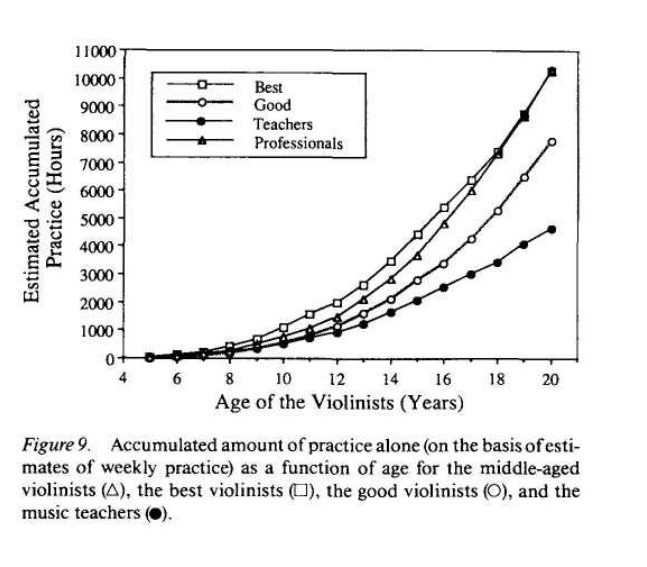
\includegraphics[width=0.5\textwidth]{berlin_practice}
      }
\end{frame}

\begin{frame}
  \frametitle{What's wrong with 10,000 hours}
  \begin{itemize}
    \item Ericsson's thesis: Monotonic improvement with deliberate practice
    \item Gladwell's thesis: 10,000 hours $\Leftrightarrow$ mastery
    \item Problems with Gladwell's thesis, according to Ericsson:
      \begin{itemize}
        \item 10k hours arbitrary number: they weren't masters yet; e.g. 20-25k for international piano competition winners
        \item Only 10k by age 20 \textit{on average}
        \item Not necessarily deliberate practice
        \item Not ``if and only if''
      \end{itemize}
  \end{itemize}
\end{frame}

\begin{frame}
  \frametitle{The takeaway}
  \begin{itemize}
    \item Not attempting to settle ``hard work vs. talent'', IQ, etc. As usual, more subtle
    \item What it means to systematically get better
    \item Surprising aspects
      \begin{itemize}
        \item Tangible reasons why people are ``good''
        \item Development of expertise: minimums
        \item Enormous capacity for improvement
      \end{itemize}
    \item 10k hours not quite correct
  \end{itemize}
\end{frame}

\section{How do machines learn}

\begin{frame}
  \frametitle{Machine learning basics}
  \begin{itemize}
      \item Three components to any ML problem: the \textbf{task}, the \textbf{performance measure} and the \textbf{data}
      \item Essential definitions
      \begin{itemize}
          \item \textbf{Features}
          \item \textbf{Model}
          \item \textbf{Parameters}
          \item \textbf{Loss}
      \end{itemize}
  \end{itemize}
\end{frame}


\begin{frame}
  \frametitle{Deep learning}
  \centering{\href{http://scs.ryerson.ca/~aharley/vis/conv/}{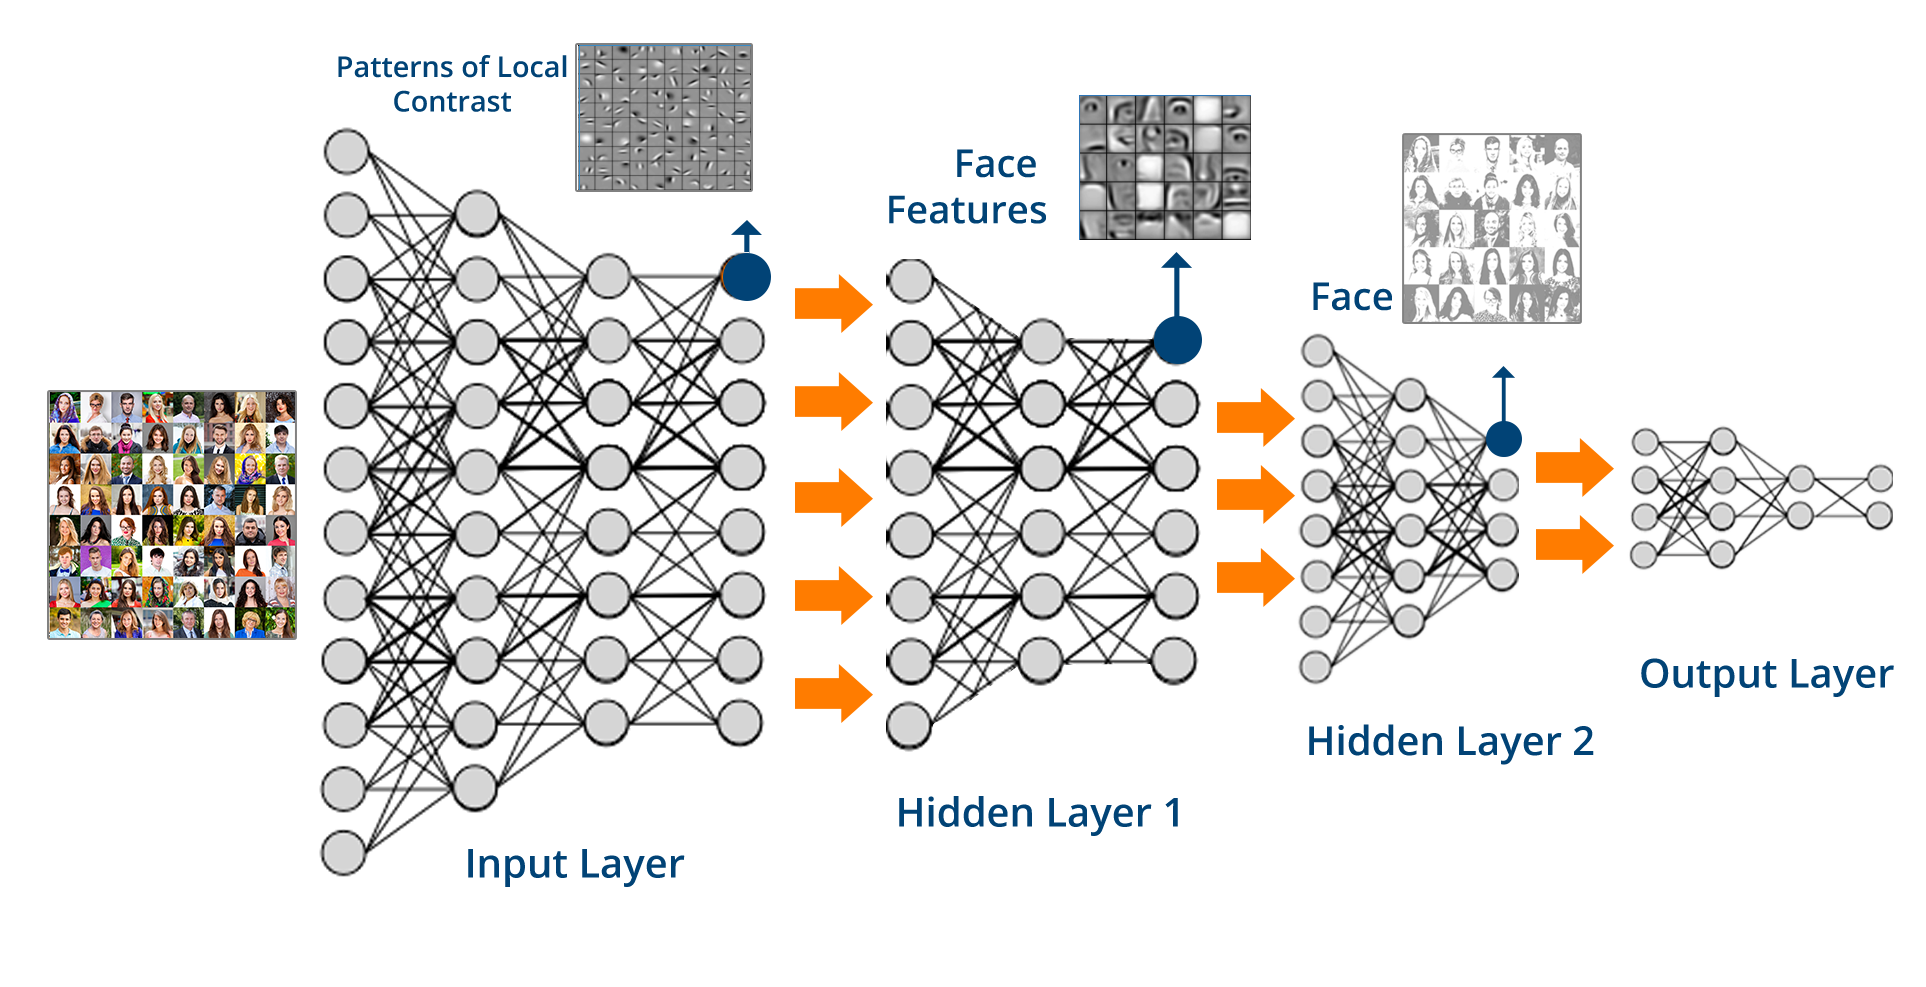
\includegraphics[width=\textwidth]{cnn.png}}}
\end{frame}

\begin{frame}{Why deep learning?}
  \begin{itemize}
    \item Probably not
      \begin{itemize}
        \item Universal approximation theorem
        \item No free lunch theorem

          {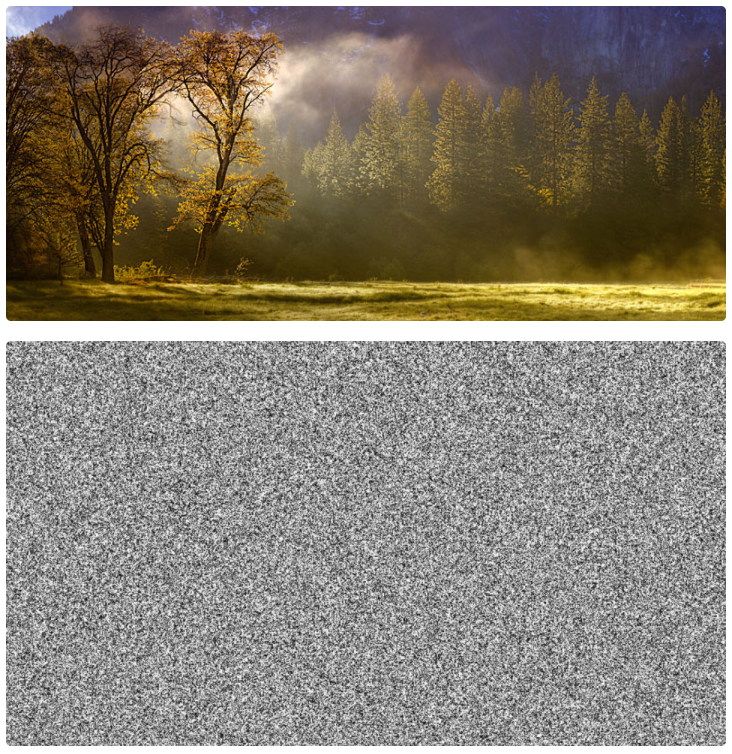
\includegraphics[width=0.2\textwidth]{nfl.png}}
      \end{itemize}
    \item Probably
      \begin{itemize}
        \item Feature learning
        \item Hierarchical representations
      \end{itemize}
  \end{itemize}
\end{frame}



\begin{frame}
  \frametitle{Optimization of a nonconvex loss function}
  \centering{
    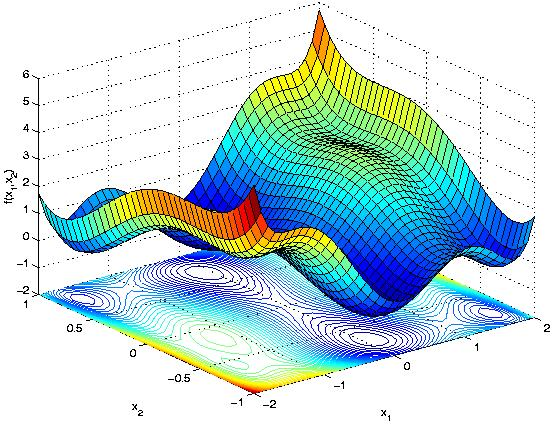
\includegraphics[width=0.8\textwidth]{nonconvex_opt.jpg}
  }
\end{frame}


\begin{frame}{Connections to human learning}
  \begin{itemize}
    \item Same sensory inputs $\Rightarrow$ different tasks $\Rightarrow$ different representations\footnote{yixinlin.net/writings//2016/10/18/representations.html}
      \begin{itemize}
        \item Chunking, ``numbers to leave numbers'': extracting relevant information, process nonlinearly, arrive at simple chunks
      \end{itemize}
    \item Feature extraction is hierarchical
    \item Deliberate practice as nonconvex optimization
      \begin{itemize}
        \item Seeking out strong gradients
        \item ``Pretrain'', understand optimization landscape through experience
        \item Local minima
        \item Surprising solutions and flexibility with consistent optimization: \href{https://blog.openai.com/faulty-reward-functions/}{OpenAI blog post}
      \end{itemize}
  \end{itemize}
\end{frame}

\begin{frame}{Takeaways}
  \begin{itemize}
    \item Humans learn expertise from deliberate practice
    \item Basics of machine learning
    \item Shared insights: learning is \textit{one concept} carried out by biology or silicon
  \end{itemize}
\end{frame}

\end{document} 
